\documentclass[12pt]{article}
 
\usepackage[margin=1in]{geometry} 
\usepackage{amsmath,amsthm,amssymb}

\usepackage[brazilian]{babel}
\usepackage[utf8]{inputenc}
\usepackage[T1]{fontenc}
\usepackage{graphicx}         %pacote para incluir figuras tipo eps
\usepackage{xcolor}
\usepackage{float} 
\usepackage{epstopdf}
\usepackage{longtable}
\usepackage{subcaption}

 
 %Matlab code in latex 
\usepackage[final]{listings}
\usepackage{color} %red, green, blue, yellow, cyan, magenta, black, white
\definecolor{mygreen}{RGB}{28,172,0}
\definecolor{mylilas}{RGB}{170,55,241}
\lstdefinestyle{myMatlab}
{
language=matlab,frame=single, basicstyle=\small\ttfamily,breaklines=true,%
morekeywords={matlab2tikz}, keywordstyle=\color{blue}, morekeywords=[2]{1}, keywordstyle=[2]{\color{black}}, commentstyle=\color{mygreen}, stringstyle=\color{mylilas}, identifierstyle=\color{black}, showstringspaces=false,%without this there will be a symbol in the places where there is a space
numbers=left, numberstyle={\scriptsize \color{black}},% size of the numbers
numbersep=9pt, % this defines how far the numbers are from the text
% emph=[1]{for,end,break},emphstyle=[1]\color{red}, %some words to emphasise
% emph=[2]{word1,word2}, emphstyle=[2]{style},
}
 
\newcommand{\N}{\mathbb{N}}
\newcommand{\Z}{\mathbb{Z}}
 
\newenvironment{theorem}[2][Theorem]{\begin{trivlist}
\item[\hskip \labelsep {\bfseries #1}\hskip \labelsep {\bfseries #2.}]}{\end{trivlist}}
\newenvironment{lemma}[2][Lemma]{\begin{trivlist}
\item[\hskip \labelsep {\bfseries #1}\hskip \labelsep {\bfseries #2.}]}{\end{trivlist}}
\newenvironment{exercise}[2][Exercício]{\begin{trivlist}
\item[\hskip \labelsep {\bfseries #1}\hskip \labelsep {\bfseries #2.}]}{\end{trivlist}}
\newenvironment{reflection}[2][Reflection]{\begin{trivlist}
\item[\hskip \labelsep {\bfseries #1}\hskip \labelsep {\bfseries #2.}]}{\end{trivlist}}
\newenvironment{proposition}[2][Proposition]{\begin{trivlist}
\item[\hskip \labelsep {\bfseries #1}\hskip \labelsep {\bfseries #2.}]}{\end{trivlist}}
\newenvironment{corollary}[2][Corollary]{\begin{trivlist}
\item[\hskip \labelsep {\bfseries #1}\hskip \labelsep {\bfseries #2.}]}{\end{trivlist}}
 
\begin{document}
 
% --------------------------------------------------------------
%                         Start here
% --------------------------------------------------------------
 
\title{Exercício 05}
\author{Renan Salles de Freitas\\
CPE 723 - Otimização Natural}
 
\maketitle


\begin{exercise}{1}
Segue o código MatLab correspondente ao EP para resolver a
função de Ackley para $n=30$, $\mu = 200$:
\lstinputlisting[style=myMatlab]{matlab/ex1/ex1.m}

Para a mutação, optou-se pela não correlacionada de n steps:
\lstinputlisting[style=myMatlab]{matlab/ex1/mutation.m}
Todos sofrem mutação.

A seleção ocorre com o critério \textit{round-robin tournament} com $q=10$, para
o conjunto pais e filhos:
\lstinputlisting[style=myMatlab]{matlab/ex1/selection.m}

Avaliando a implementação 100 vezes e calculando-se a média e desvio padrão,
obtemos:
\begin{align*}
J_{\text{medio}} &= 16.4641 \\
J_{\text{std}} &= 2.4430 \\
J_{\text{min}} &= 2.1270
\end{align*}

Mostrando que a recombinação é importante para este problema, já que o
desempenho foi bem pior.
\end{exercise}

\begin{exercise}{2}
Na implementação dos EA clássicos (baunilha) o número de avaliações da função
custo é fixo em cada geração. Por exemplo, no exercício 1 acima, o número de
avaliações da função custo é $2 \times \text{tamanho da população}$ por geração.
Dessa forma, nos algoritmos clássicos, avaliar a velocidade do EA por número de
gerações é semelhante a avaliá-lo pelo número de vezes que a função custo é
computada.
\end{exercise}

\begin{exercise}{3}

Os algoritmos genéticos buscam um equilíbrio entre exploração global e local,
isto é, explorar a área de busca tanto quanto possível, e concentrar a
exploração em torno de um ponto (mínimo global).

Em algoritmos genéticos, a mutação é o passo que tenta evitar a convergência e
explorar mais a área de busca. Nos algoritmos, faz sentido explorar mais a
área de busca no início, nas gerações iniciais (assegurando a diversidade da
população) e, nas últimas gerações, o algoritmo tenta reduzir a área de busca,
explorando próximo ao mínimo global. Nessa estratégia, o parâmetro de mutaçãoo
cai com o número de gerações. Há, porém, um problema comum nessa estratégia.
Quando a população converge para um mínimo local, o algoritmo deveria aumentar
a diversidade da população, explorando outras áreas. Esses dois comportamentos
são justificativas de porque os parâmetros da mutaçãoo devem ser aumentados e
reduzidos conforme as gerações.
\end{exercise}

\begin{exercise}{4}
Foi implementado um ES para resolver o problema de \textit{clustering} em
$\mathbb{R}^2$. O código MatLab segue abaixo:
\lstinputlisting[style=myMatlab]{matlab/ex4/ex4.m}

Os parâmetros escolhidos podem ser vistos no código. Após 1000 gerações,
obtivemos $J_{\text{min}}=0.3889$. A figura abaixo mostra a situação final.

\begin{figure}[H]
    \centering
    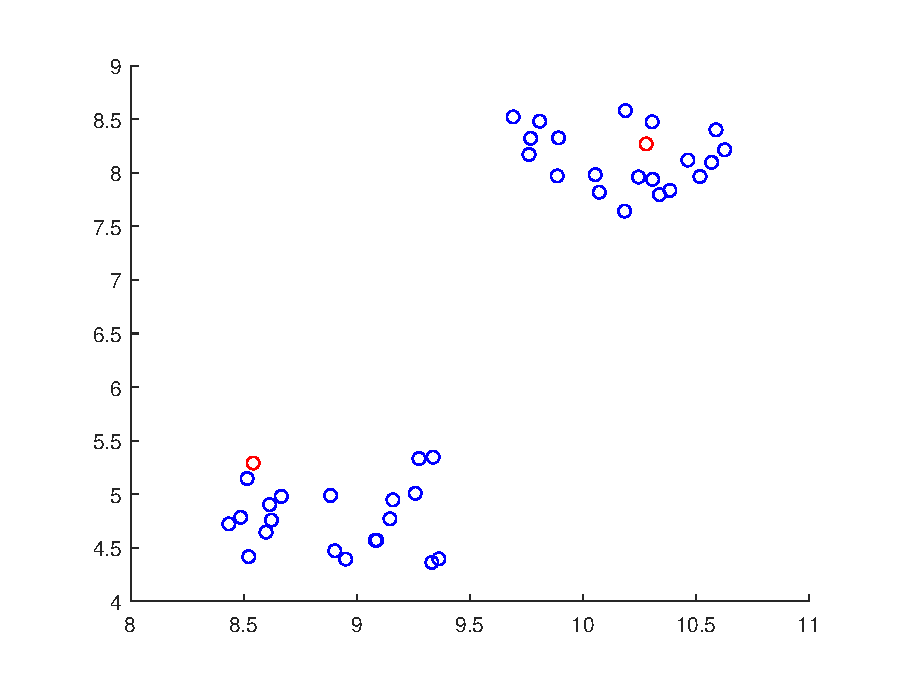
\includegraphics[width=0.5\textwidth]{figs/cluster.eps}
\end{figure}

\end{exercise}


\end{document}
              
